%!TEX root=../main.tex
\chapter{Background}
\label{ch:background}
This chapter explains the background for this thesis. Section \ref{sec:mbp} introduces the Mont Blanc Project, the project goals and its current status, as well as the largest and most significant prototypes.

\section{The Mont Blanc Project}
\label{sec:mbp}
The \gls{mb} \cite{m:MB} started in October 2011. The project received 14 million Euros as initial funding, and 8 of those millions were granted by the European Commission. The project received an additional funding of 8 million Euros from the European Commission after two years. With a total funding of 22 million Euros, it was estimated that the project would last until September 2016. The project has also been extended as of October 2015, with an extension budget of 7.9 million Euros funded by the European Commission. As mentioned in section \ref{sec:mot}, the long-term goal is to reach Exascale performance using 15 to 30 times less energy than other HPC systems. The energy performance metric used is FLOPS/W, motivated by the Green500 list \cite{m:Gr500}. The project is split into three phases; the first two coordinated by the Barcelona Supercomputing Center \cite{m:bsc}, while Bull \cite{m:bull} coordinates the third phase.

\subsection{Project Goals and Status}
Both Ramirez \cite{m:MB-PRACE-14} and Mantovani \cite{m:MB-15} has summarized the goals of the first two project phases. Mont-Blanc phase 1, valid from 2011 to 2015, had three main objectives. The first was to deploy a prototype scalable to 50 PFLOPS with a total power consumption of 7MW using the available energy efficient embedded technology, which should be competitive with the Green500 leaders of 2014. The second objective was to overcome some limitations found during development and use the gained knowledge in the design of the next generation HPC system. They aimed for a HPC architecture that should be scalable to 200 PFLOPS on 10 MW, which should be competitive with the Top500 leaders of 2017. The third and last objective was to port and optimize Exascale scientific applications capable of exploiting the new generation HPC systems described in objective 2. \\*

The \gls{mb} phase 2 valid from 2013 including September 2016 has 4 objectives. The first objective is to supplement the Mont Blanc prototype software stack with software development tools and support ARMv8 \gls{isa}. The second goal is to construct the initial definition of the Exascale architecture, which involved deployment of small ARM-based mini-clusters and evaluation of their suitability in \gls{hpc}. Objective number three is to be up to date with newly released ARM products and evaluate if they are suitable for \gls{hpc} architectures. The last and fourth objective is continued support for the Mont Blanc project. These objectives is also summarized by Follan and Støa \cite{mt:T&S} and on the \gls{mb} website \cite{m:MB}.\\*

Mantovani reported the project status in July 2015 \cite{m:MB-15}. Among the tasks finished so far is the deployment of a software stack to support the Mont Blanc system (see prototype below), porting of new HPC kernels and applications, and design, development, deployment and monitoring of the Mont Blanc prototype. Amidst the ongoing work is ARM 64 bit exploration, porting new applications for the HPC architecture developed, enhance the programming model (OmpSs \cite{m:ompss}) used and monitor the Mont Blanc prototype for fault tolerant techniques. \\*

The third phase of the project started in October 2015. The goal is to design a new HPC platform that is able to improve the performance-energy ratio when executing actual applications. This will be done by using a co-design approach, which will ensure that hardware and system innovations are transformed into HPC application benefits.

\subsection{Prototypes}
Multiple prototypes have been announced, and the specifications of the most significant prototypes are listed below:
\begin{enumerate}
\item \textbf{Tibidabo} \cite{a:MB:Tib}: Tibidabo is the first prototype of the MB project. The prototype is an experimental system and a proof-of-concept HPC system, to show that it is possible to deploy a large scale HPC cluster using ARM processors. The prototype contains compute boards with NVIDIA Tegra 2 SoC, with dual core ARM Cortex A9 @ 1GHz. The GPUs on the chip did not support the standard programming models OpenCL and CUDA, and were therefore not used in the cluster. However, the compute cards can be replaced with up-to-date chips as they become available with updated GPUs that support the two programming models. The prototype consists of 128 nodes each containing a Q7 module, each module hold a Tegra 2 chip. The prototype achieves 120 MFLOPS/W on High-Performance Linpack (HPL) benchmarks.
\item \textbf{Pedraforca} \cite{m:MB:Pedr}: Pedraforca consist of combination of ARM processors and NVIDIA GPU's. One compute node consists of a NVIDIA K20 GPU and a Tegra 3 Q7 Module containing 4 ARM Cortex A9 @ 1.3 GHz. The system contains 78 such compute nodes. It is the first large scale HPC system that makes use of ARM-based processors. Even though some factors of the initial technology stack limits the system, the prototype contributes towards the use of ARM-based embedded processors in \gls{hpc} systems.
\item \textbf{Mont Blanc} \cite{m:MB:MB-prot}: The latest prototype from the MB project (updated specs in 2015 \cite{m:MB-15}). The system contains a rack with a total of 1080 Exynos 5 compute cards, or  2160 ARM Cortex-A15@1.7 GHz CPUs, 1080 ARM Mali T604 GPUs, 4.3 TB of RAM and 17.2 TB of Flash memory. The performance is about 35 TFLOPS and the power consumption is about 24 kW. In November 2014, the Mont Blanc Prototype had an energy efficiency of 1.5 GFLOPS/W. The best Green500 ranking during that time was approximately 5.2 GFLOPS/W.
\end{enumerate}



\section{The Climbing Mont Blanc Project}
Climbing Mont Blanc (CMB) is an Online Judge focusing on energy efficient programming on ARM based platforms, greatly inspired by the Mont Blanc project. An Online Judge is a web application or web based woftware system which let its users upload programming solutions to defined set of programming problems. Most Online Judges serve problems with varying degrees if difficulty, and can compile and run multiple programming languages (see more in chapter \ref{ch:related}). The paper "\textit{Climbing Mont Blanc - A Training Site for Energy Efficient Programming on Heterogeneous Multicore Processors}" \cite{a:CMB} describes the CMB system. The first version of CMB was developed by Torbjørn Folland and Simen Støa during their Master thesis during the Spring of 2015 \cite{mt:T&S}. The source code is available on \textit{Bitbucket} \cite{m:bitbucket}, which uses \textit{git} \cite{m:git} version control.

\subsection{Architecture}
The architecture of CMB is shown in figure \ref{fig:cmb_arch}. As seen by the figure, the system consists of three main parts; the \textit{frontend}, the \textit{server} and the \textit{backend}. The three parts are explained in detail below.

\begin{figure}
  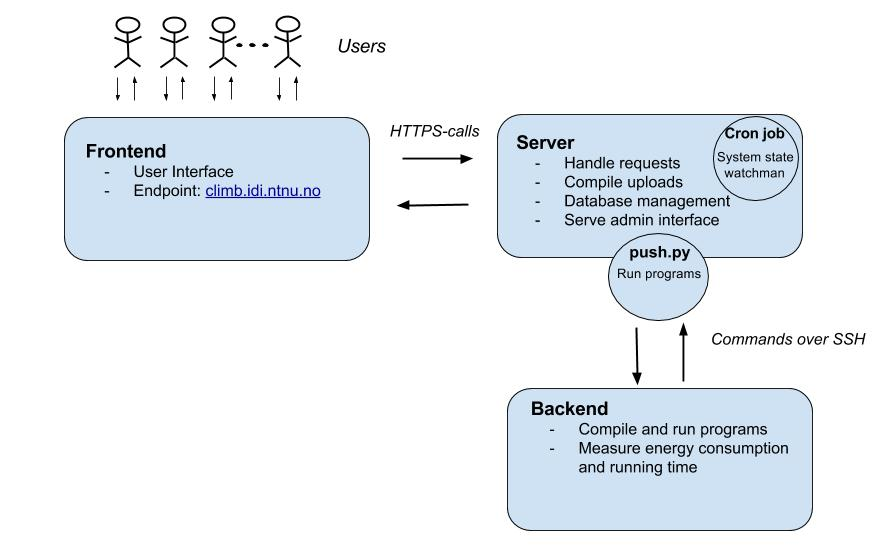
\includegraphics[width=1.0\textwidth]{figs/cmb_arch.jpg}
  \caption[The Climbing Mont Blanc system architecture]{The Climbing Mont Blanc system architecture}
  \label{fig:cmb_arch}
\end{figure}

\subsubsection{Frontend} The user interface and handles all user based interaction. The frontend is written in Javascript (ECMAScript $5^{th}$ Edition) and AngularJS \cite{m:angular}. AngularJS is a framework developed by Google and are now maintained by Google and individual developers. The framework is built according to the Model View Controller pattern and extends HTML with dynamic views with two-way data binding for building single page applications. The result is a smoother user experience, as the page updates the views dynamically with no need of refreshing the web-page. The framework also lets the developer define own reusable components, which in most situations make the code base more structred. The view structure is defined in HTML5 while CSS3 takes care of the view styling. Google Analytics monitors the frontend, which is an advanced monitoring software provided by Google. There is a vast number of things that can be monitored and analyzed. Among the things monitored is the number of users, number of new users and user behavior. Chapter 5 of Torbjørn and Simen's Master Thesis contains more information about system monitoring, and a detailed description of the technologies used \cite{mt:T&S}. \\

The system frontend can be reached at \url{https://climb.idi.ntnu.no}. In this paragraph, \textit{navigate} means to perform an action to change the view in the user interface. The views change according to user state, and views updates and changes when performing actions against the system. As an example, navigating to the view of a specific problem   like login, sign up, create and join groups view, view the \textit{HowTo}-page, view problems and navigate to a specific problem to solve. If the user navigates to a specific problem, the view differs depending on the state of the user. If the user is not logged in, it may only view the submitted programs that are set to be \textit{visible}\footnote{A user may change the visibility of their submissions and results through the user interface.}. The user may upload programs if they are signed-in, and if so the problem view is changed to make it possible to upload files. The file uploaded currently needs to be a zipped folder containing the source code. Further usage information of the system are found in Appendix \ref{appendix/paper} and the Master Thesis of Follan and Støa. \\

\begin{figure}
    \centering
    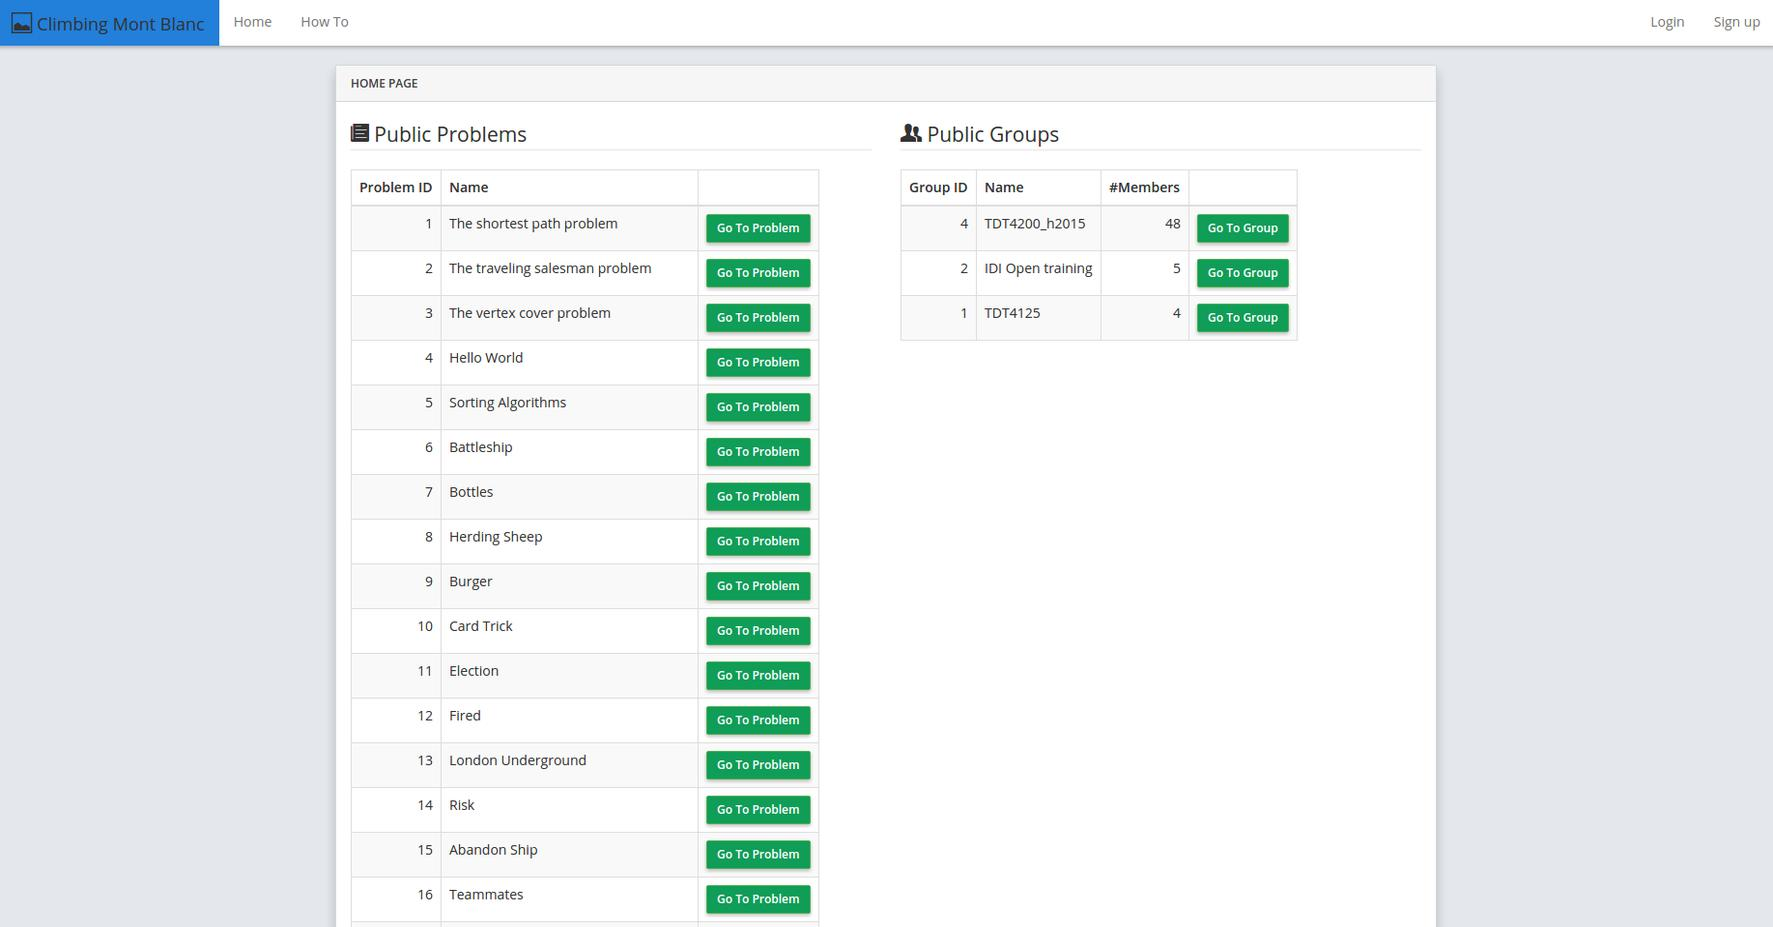
\includegraphics[width=0.8\textwidth]{figs/front_page.jpg}
    \caption[Climbing Mont Blanc Home Page]{Climbing Mont Blanc Home Page}
    \label{fig:front-page}
\end{figure}

\subsubsection{Server} The server is implemented as an REpresentional State Transfer (REST) Application Programming Interface (API), as defined in by Roy T. Fielding et.al \cite{a:rtf}. The RESTful API is implemented using Python Flask \cite{m:flask}. The server also makes use of Gunicorn \cite{m:guni} to handle simultaneous requests from multiple users. On our development and production servers, Nginx \cite{m:nginx} is also used as a \textit{reverse proxy}. It serves static files on the fly while requests for dynamic content (updated submissions etc.) are forwarded to Gunicorn. SQLite \cite{m:sqlite} is used as database with SQLAlchemy\cite{m:sqlalc} on top. SQLAlchemy functions as an Object Relational Mapper (ORM) that is it associates Python classes with database tables and objects of those classes with rows in the tables. SQLAlchemy makes it easy to interact with the database, as one only modify object structures. The server runs within a Python \textit{Virtual environment} \cite{m:virtualenv}, which have all Python required dependencies\footnote{Dependencies is meant by dependencies in between packages (read: code libraries). As an example, SQLAlchemy might require a specific version of Python Flask installed in order to work correctly.} installed within a virtual environment. The virtual environment contains only the packages needed by the server, which removes potential dependency errors if other Python based systems also runs on the server. The server is responsible for handling requests from the client, storing useful information in the database (like submissions) and compiling submitted programs. A Python program called \textit{push.py} is run in the background, constantly checking a run queue for runnable programs. If there is a program ready to run in the queue, the script will push the program over to the backend, and then compile and run it using SSH. The result is then returned to the server, and the server checks the correctness of the program before reporting the result back to the frontend. Finally, the server is responsible for checking the state of the system with a background cron job. The cron job runs every 15 minutes, checking if the three parts Gunicorn, \textit{push.py} and backend is up and running. The system sends out an automatic e-mail in case of system failure. \\*

The server also provides and administrator interface. Admin users have special privileges which grants them access to the admin interface found at \url{http://climb.idi.ntnu.no/admin}. Procedures that modify the database or the server file system are all done through the admin interface. The admins can control a lot of the content visible on the frontend, such as programming problems visibility. The most common administrator opration is to add new problems, which requires the admin to add a new problem to the database and upload all files needed to the server. The files needed to make a problem solvable is the input files to be piped into the submitted programs, files that holds the expected result of a execution and a special file called \textit{checker.cpp} that checks the correctness of submitted programs. When a program is executed, the input files are given as arguments to the submitted program. When the program is done executing, the checker compares the output of the submitted program against the expected answer files. The program is accepted if the output passes the checker program. Since the checker is a regular C++-program, it is up to the admin to define what sort of output that should be accepted by the checker. Most of the problems available simply checks the difference between output and expected output using the Unix \textit{diff} program. A special database field called \textit{goodness} can also be added to the problem. The database field is meant for approximation problems to check how "good" a solution is. As an example, a solution to the Vertex Cover problem might yield a different cover on each run. The admin making the problem can then define in the checker if a given cover size is good or not.

\subsubsection{Backend} The executing unit of the CMB system. It is an Odroid XU3 board \cite{m:odroid} which consists of an Exynos 5 Octa heterogeneous multicore. A block diagram of the board is shown in figure \ref{fig:odroid-block}. CMB only uses a minimal of the external interfaces and components on the system: the Ethernet port for internet access, eMMC module or MicroSD card for the OS and file system and the board energy monitors. The Exynos 5 Octa consists of four big ARM Cortex A-15 and four small ARM Cortex A-7 cores. Both CPU types have the same Instruction Set Architecture (ISA), but they have different characteristics when it comes to performance and power consumption. The Exynos chip also has an ARM Mali-T628 GPU with six cores. With the two ARM processor types and the Mali GPU, the chip can be called a \textit{three way heterogenous multicore with 14 cores}. The cores also use the ARM big.LITTLE technology, which makes it possible for the Operating System (OS) to perform Global Task Scheduling, that is to dynamically assign threads to the most appropriate CPU based on the run-time information \cite{m:big-little}. The board will compile and run the programs pushed over to it by \textit{push.py}. While running uploaded programs, the board will measure time and energy (see subsection \ref{sec:em-cmb}). When the board finishes running and calculating energy consumption for a given program, it will send the result back to the server for further processing. The observant reader might view a compilation both at the server and at the board as redundant. First, there is a lack of good enough cross-compiler. Second, the compilation at the server gives quicker feedback to the user in case of compilation errors. The CMB system currently supports the programming languages C and C++, compiled with gcc-4.9 and g++-4.9 respectively. The compilers have support for both OpenCL v1.1, OpenMP 4.0 and PThreads NTPL 2.19.

\begin{figure}
    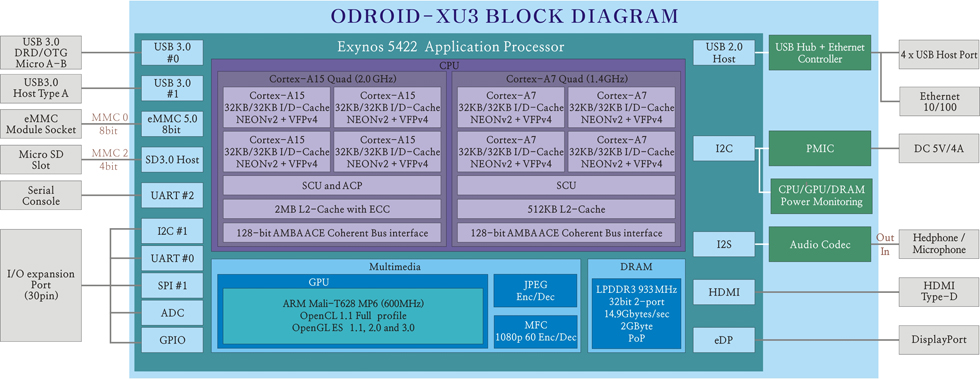
\includegraphics[width=1.0\textwidth]{figs/block-xu3.jpg}
    \caption[Odroid XU3 Block Diagram]{Odroid XU3 Block Diagram (source: Hardkernel Website \cite{m:XU3-block})}
    \label{fig:odroid-block}
\end{figure}

\subsection{Energy Measurements}
\label{sec:em-cmb}
The Hardkernel EnergyMonitor program that is compatible with the Odroid XU3 is used to monitor the energy consumption of the submitted programs. The pipeline in figure \ref{fig:pipeline} presents the execution pipeline for the backend on submission of a program. When a program is to run, it is first compiled and then run with small input to check for runtime errors. If there are no runtime errors, the EnergyMonitor program is started. The cache is then cleared and the CPU is heated using the UNIX \textit{stress} \cite{m:stress} command. Clearing the cache is done due to irregularities in energy readings which were a bug discovered during the Spring 2014. The CPU runs \textit{stress} to obtain a stable target temperature (currently 60 degrees Celsius) before running the program as it might also have an effect on energy readings, as proposed by Juan M. Cebrian and Lasse Natvig \cite{a:JL:T}. For a discussion of this matter, consult Follan and Støa's Master Thesis \cite{mt:T&S}. The current backend uses the sensors monitoring the temperature of the four big ARM Cortex A15 cores to arrive at the given target temperature of 60 degrees. The program is then run, and finally the EnergyMonitor program stops and the result is reported back to the server as seen in the figure. \\

Right before and right after a program has run, timestamps measure the time spent to execute the whole program. As seen by figure \ref{fig:pipeline}, the EnergyMonitor program is started before the running of the submitted program. To ensure accurate energy readings, the timestamps used to measure running time is also used to fetch the correct energy measurements from the output of the EnergyMonitor program.  As mentioned, when the program finishes, the monitoring stops and the energy consumption is calculated and returned to the server. The server then calculates the Energy Delay Product (EDP), which is the main energy metric used in CMB, as it emphasizes both energy and performance \cite{b:edp}. Energy is in itself not a good energy metric, since we could simply run a program on a slow and under clocked CPU to obtain low energy consumption. EDP is defined in equation \ref{eq:edp}, where \textit{E} is the energy used, \textit{D} is the delay or execution time.

\begin{equation}
  \label{eq:edp}
  EDP = E * D
\end{equation}

By comparison, the Mont Blanc project uses the metric FLOPS/W. This metric may be a good metric when running the same benchmark (that is the same implementation) over and over again to test a system architecture. However, CMB compares different implementations of known problems. Because of these limitations it is difficult to use the FLOPS/W metric in the CMB system, as the number of operations may differ from one implementation to the next. Another problem is to determine the number of \textit{useful} instructions, that is instructions that contribute towards solving the problem. For these reasons, it is much easier to use EDP as energy metric.

\begin{figure}
  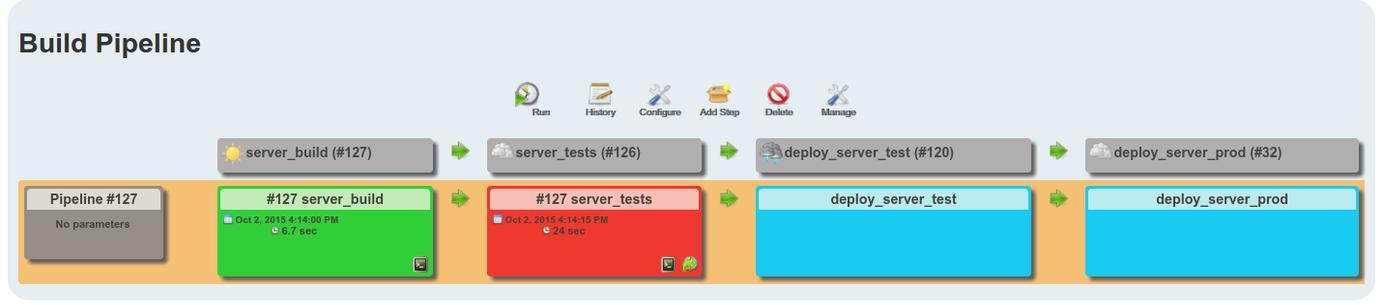
\includegraphics[width=1.0\textwidth]{figs/server_pipeline.jpg}
  \caption[Server Build Pipeline]{Server Build Pipeline}
  \label{fig:server-ci}
\end{figure}

\subsection{Code Correctness and System Environment}
To quickly deploy new versions of the code, the system makes use of \textit{Jenkins} \cite{m:jenkins} as Continuous Integration (CI) server or build server. CI is a software engineering practice that automates the testing and deployment of systems. Some benefits of CI is reported by Fowler in his article from 2006; a clone of the production environment (so-called development server) runs tests on the code change before deployment to production, bugs are discovered and removed easily, and as a whole it makes it possible with rapid integration of new features \cite{a:F:CI}. The CMB development server has the a Jenkins server installed. It is easier to describe what CI and Jenkins are with a description with a example from the CMB system as below. Jenkins makes it easy to define \textit{build pipelines}. Each build pipeline consists of \textit{jobs} and \textit{triggers}. A job can among many things pull code from a Bitbucket repository, execute scripts, execute scripts over SSH, or \textit{trigger} other jobs. An example build pipeline is shown in figure \ref{fig:server-ci}, which shows the build pipeline for the server. The execution of the pipeline starts with sensing a change in the Bitbucket repository and pulling the newly changed code. The job then installs all Python requirements with \textit{pip} \cite{m:pip}, which is the Python package manager (within the virtual environment as explained above). It then triggers the next job, which is the running of \textit{automatic unit tests} with \textit{nose} \cite{m:nose} and \textit{linting}\footnote{Linting is the automatic process to uncover errors and to ensure some coding standards.} with \textit{flake8} \cite{m:flake}. If the testing and linting passes, the job then triggers the next. The next job automatically deploys and set up the test server for further manual testing by executing scripts over SSH. The code is run in with debugging enabled, such that logs are available when doing manual tests. One can trigger the next job manually, which deploys the change to the to the production server. The deployment to production involves both setting up the frontend and backend for production and restarting the server. The frontend code is set up with minimized and concatenated HTML, CSS and Javascript files to improve performance. \\

\begin{figure}
  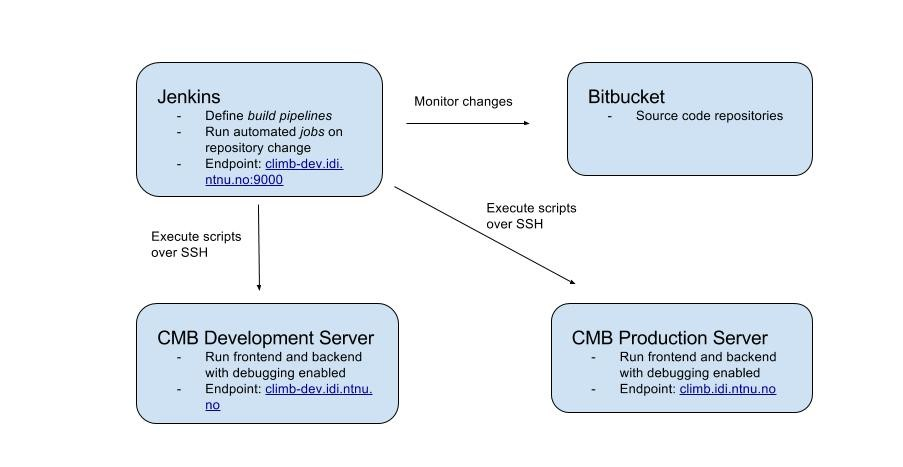
\includegraphics[width=0.9\textwidth, height=0.5\textwidth]{figs/server_env.jpg}
  \caption[CMB Server Environment]{CMB Server Environment}
  \label{fig:cmb-server}
\end{figure}

The frontend build pipeline has a similar procedure. The only difference is minor changes in the commands run by Jenkins. The first job pulls code from the Bitbucket frontend repository if a change has happened, and install all requirements with the package manager \textit{npm} \cite{m:npm}. It then runs the frontend code linter, \textit{jshint} \cite{m:jshint} for Javascript code, and sets up the frontend in debug mode (developer mode) through a tool called \textit{gulp} \cite{m:gulp}. Gulp is a build system that enables the programmer to define \textit{tasks} that may consist of multiple commands to achieve some goals. The goals of this step are first to run the task of running the linter and then run the task of building the source code with debugging enabled. If the Jenkins job is successful, the next job in the pipeline is triggered. The second step makes use of another package manager called \textit{bower} \cite{m:bower}, which installs dependencies used in the unit tests for the frontend. The Jenkins job then executes the automatic tests with gulp. If the automatic unit tests are successful, a third Jenkins job is triggered. The job simply deploys to the CMB development server, by pulling all changes, installing all requirements with \textit{npm}, and finally setup the frontend in debug mode through a task in gulp. To deploy to the production environment, one can manually trigger the Jenkins job like on the server pipeline. The job deploys the code change to the CMB production server, much like the Jenkins job for deploying to production. The only change is that it only sets up the frontend, it does not do a full server restart like above. The figure \ref{fig:cmb-server} summarizes the server environment and the interactions between each of the CMB servers with Jenkins. The observant reader might see that the workflow is the same for both pipelines. First Jenkins setup the code, then it runs automatic unit tests, then deploys to the development server, and lastly may manually deploy to the production server. When a change happens in the Bitbucket repository (some developer have developed new code) launches Jenkins and the workflow is executed. All development should be done locally, it is considered bad practice to develop new features on either the development or production server.

\subsection{Security}
\paragraph*{User Information Security}
%User specific information is stored in the database. Among the information stored is the user name and password of all users. The password itself is ran through a method called \textit{generate\_password\_hash} \cite{m:gph}, which is part of the Python \textit{Werkzeug security} package, upon user creation. This ensures that the password is hashed before stored in the database. The admin users also have similar hashed passwords stored in their table in the database. The same password will generate the same hash every time, but it is not possible to reconstruct the password from the hashed password found in the database. The password is sent and checked upon login, and if the password hash matches the hash in the database, a \textit{token}\footnote{A token is some unique string valid for a specific period of time} is sent back to the user. This token contains enough information to uniquely describe a user session. The token is sent in the HTTP Authorization Request Header, which makes it possible for the server to return user specific information. The token is valid for one hour, which means that a user can be inactive up to one hour. After the token expires, the user needs to log back in to access user specific information. The token is stored at the frontend, which makes the server stateless. To make the transfer of information more secure, the HTTPS protocol is used to encrypt all information sent in a request. HTTPS makes use of Secure Socket Layer (SSL) encryption, which makes it almost impossible to decrypt messages sent from the server. For example, fetching a user name or password during log in or user creation will be hard to achieve.

\paragraph*{Uploaded Programs Security}
%Programs uploaded can potentially contain malicious code or file names. It is hard to predict if the uploaded code is malicious or not, and it is easier to restrict the permissions of the user running the uploaded program. The solution is to let a user with as few permissions as possible run the uploaded program. The CMB backend therefore has a user called \textit{worker} for that purpose. To secure and remove potential threats residing in the file name, the Python Werkzeug security procedure \textit{secure\_filename} \cite{m:sf} is used before storing the uploaded file. The system also uses a predefined Makefile to compile the uploaded programs. If an unknown error occurs, it might crash the server. One way of making the server more secure and stable in such cases, is to have a separate compile server or thread. If the compilation server crashes unexpected, the system still stays active to handle more requests. This has not been implemented, since no such problem has occurred.

\paragraph*{System Security}
%As mentioned, to secure the messages sent, HTTPS is used which encrypts and decrypts messages with Secure Socket Layer (SSL). The reverse proxy used at the servers, Nginx, is configured to handle HTTPS requests. SSL requires a SSL Certificate to work, which is a guarantee that the holder of the certificate is trustworthy. Most browsers has a list of Certificate Authorities (CA), which is some third party issuing the certificates. Uninett created the certificate that is used by the CMB system which is known by most browsers. The messages sent from CMB is therefore trusted. The backend of CMB also has Uncomplicated Firewall (UFW) \cite{m:ufw} installed, which restricts access to the board. The firewall requires every SSH requests to come from within the NTNU network itself, which means that the backend is only accessible from NTNU or through a Virtual Private Network (VPN). The backend also has Fail2ban  \cite{m:f2b} installed, which restricts the number of authentication attempts made within a certain time-frame. If there are more than three attempts within the configured time-frame, the IP sending the requests is banned for 10 minutes. The server also has UFW and Fail2ban installed, but the setup of UFW is slightly different. UFW on the server let's all requests to port 80 and 443 be open for all requests, to enable the use of HTTP and HTTPS respectively. This makes sure that the CMB frontend is accessible from outside the NTNU network. To keep up to date with security updates \textit{unattended-updates} \cite{m:uau} is enabled, which installs security updates if needed. This is done at 02:00, which also automatically restarts the CMB system.

\subsection{Planned extensions}
Extensions to be made this spring and in the future.
Simon Holbacka++ for accurate energy readings.
